\section{Architecture}

The architecture of the UAV based SDN system for wireless sensor networks.

\begin{figure}[htbp]
	\centering
	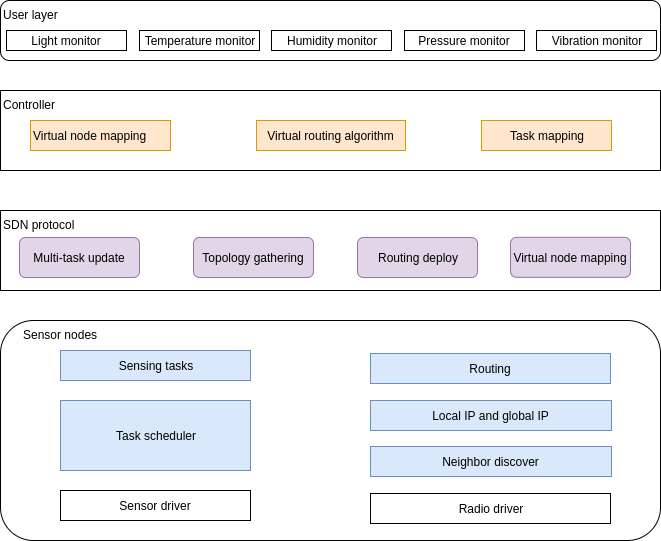
\includegraphics[width=3.5in]{./Figure/Architecture}
	\caption{Architecture of the system.}
	\label{Architecture}
\end{figure}



\begin{table}[htbp]
	\caption{System API}
	\label{API}
	\centering
	\scalebox{0.9}{
	\begin{tabular}{|l|l|}
		\hline
		\makecell[tc]{\textbf{Function}} & \makecell[tc]{\textbf{Description}} \\
		\hline
		\multicolumn{2}{|c|}{\textbf{Sensor Control API}}\\
		\hline
		\textbf{switch\_sensor(node,state)} & Turn on or turn off the sensor \\
		\hline
		\textbf{get\_sensor\_info(node)} &\makecell[tl]{ Get sensor's information, including \\ sensor's position, duty cycle, power, etc.}\\
		\hline
		\makecell[tl]{\textbf{set\_sensor\_attr} \\ \textbf{(node,attribute,value)}} & \makecell[tl]{Set node attribute, including  duty cycle,\\ radio strength, etc.} \\
		\hline
		\textbf{get\_neighborlist(node)} & Get the neighbor list of a node \\
		\hline
		\multicolumn{2}{|c|}{\textbf{Application API}}\\
		\hline
		\multicolumn{2}{|c|}{\textbf{Routing protocol}}\\
		\hline
		\textbf{topology get\_topology()} & Get the topology of the network\\
		\hline
		\textbf{set\_route(route)} & Set the routing table \\
		\hline
		\multicolumn{2}{|c|}{\textbf{Node selection}}\\
		\hline
		\textbf{nodeset naive\_selection(location)} & Select sensor set by location information\\
		\hline
		\textbf{nodeset AI\_selection(dataset)} & \makecell[tl]{Select sensor set by AI algorithm based\\ on sensing data}\\
		\hline
		\multicolumn{2}{|c|}{\textbf{Task scheduler}}\\
		\hline
		\textbf{task\_buffer(task)} & Add a new task to task buffer \\
		\hline
		\textbf{task\_schedule(buffer)} & Schedule the tasks in the buffer\\
		\hline
		\multicolumn{2}{|c|}{\textbf{Network monitoring and visualization}}\\
		\hline
		\textbf{float get\_node\_energy(node)} & Get node energy \\
		\hline
		\textbf{int get\_traffic\_num(node)} & Get traffic number\\
		\hline
		\textbf{show\_network\_info()} & Show the network GUI\\
		\hline
	\end{tabular}
	}
\end{table}

\begin{lstlisting}[language={[ANSI]C},label=update,caption={An example of deploy routing algorithm},keywordstyle=\color{blue!70},showstringspaces=false, commentstyle=\color{red!50!green!80!blue!70},frame=single,captionpos=t, rulesepcolor=\color{red!20!green!20!blue!20}]
topology = get_topology();
//calculate routetable for each node 
//based on topology 
for(node in nodeset){
	node.routetable = 
		calculate_route(topology);
}
//set route for each node
for(node in nodeset){
	UAV fly to node;
	for(route in node.routeTable) 
  		set_route(route);
}

\end{lstlisting}

